\renewcommand{\arraystretch}{1.5}
\begin{longtable}{
    |p{4cm}
    |p{5cm}
    |p{5cm}|
}
\caption{Comparativa de sensores para medición de temperatura.}
\label{tab:sensor_temperatura} \\
\hline
\textbf{Característica} 
    & \textbf{DS18B20 Sumergible \cite{DFRobot_DS18B20}} 
    & \textbf{Atlas Scientific EZO-RTD™ \cite{Atlas_EZO_RTD}} \\ 
\hline
\endfirsthead

\hline
\textbf{Característica} 
    & \textbf{DS18B20 Sumergible \cite{DFRobot_DS18B20}} 
    & \textbf{Atlas Scientific EZO-RTD™ \cite{Atlas_EZO_RTD}} \\ 
\hline
\endhead

\hline
\multicolumn{3}{r}{\textit{Continúa en la siguiente página}} \\
\endfoot

\hline
\endlastfoot

Tipo de tecnología 
    & Sensor digital 1-Wire 
    & RTD PT-1000 industrial \\ \hline

Rango de medición 
    & -55\,\textdegree C a +125\,\textdegree C 
    & -200\,\textdegree C a +850\,\textdegree C \\ \hline

Precisión típica 
    & $\pm$0.5\,\textdegree C (-10\,\textdegree C a +85\,\textdegree C) 
    & $\pm$0.1\,\textdegree C \\ \hline

Tipo de salida 
    & Digital (1-Wire) 
    & UART / I2C \\ \hline

Voltaje de operación 
    & 3.0--5.5 V 
    & 3.3--5.5 V \\ \hline

Compatibilidad con ESP32 
    & Sí (1-Wire) 
    & Sí (UART/I2C) \\ \hline

Diseñado para inmersión continua 
    & Sí 
    & Sí \\ \hline

Calibración necesaria 
    & No 
    & No \\ \hline

Costo aproximado 
    & \$7.5 USD 
    & \$30 USD \\ \hline

Ventajas 
    & Muy económico, fácil integración, adecuado para monitoreo de calidad de agua 
    & Altísima precisión, robustez industrial \\ \hline

Desventajas 
    & Menor precisión que RTD, rango limitado para aplicaciones extremas 
    & Alto costo, integración más compleja \\ \hline

Imagen
    & \shortstack{\\ 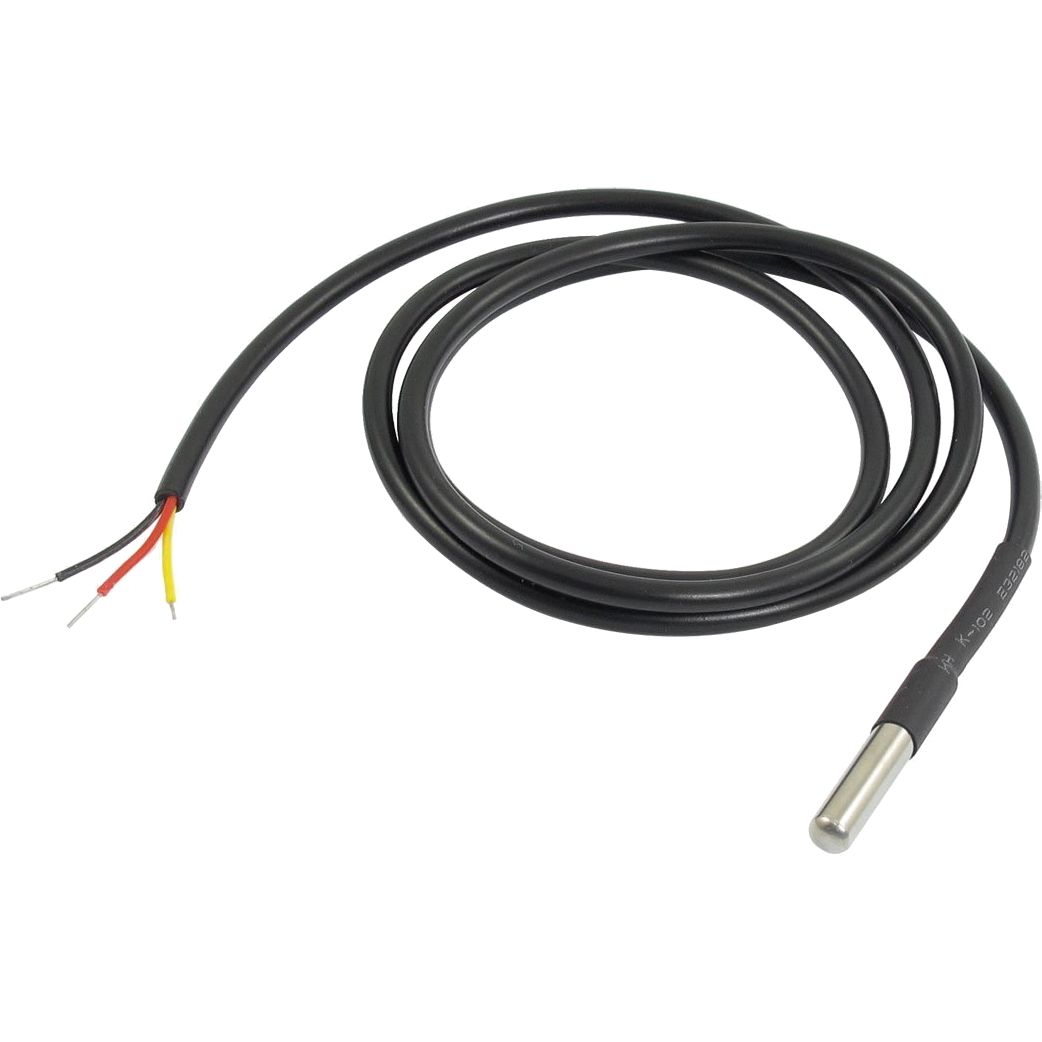
\includegraphics[width=0.75\linewidth]{Documento/Imagenes/Análisis/sensores/Temp_Sensor.png}}
    & \shortstack{\\ 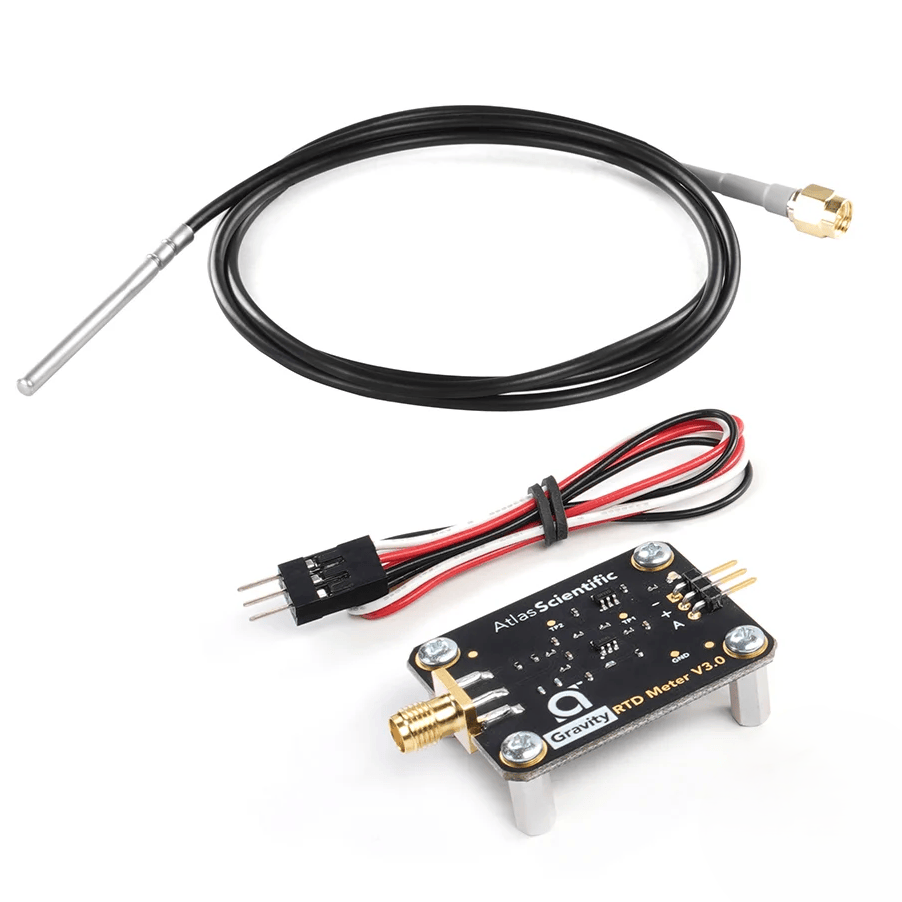
\includegraphics[width=0.75\linewidth]{Documento/Imagenes/Análisis/sensores/Temp_Atlas_Sensor.png}} \\ \hline

\end{longtable}
